
\section{Uvod}
\hspace{\parindent} Algoritam kukavičjeg pretraživanja \cite{gandomi2013}  (CSA) metaheuristički je optimizacijski algoritam utemeljen na parazitskom ponašanju nekih vrsta kukavica i slučajnoj šetnji (L\'evyjevom letu.) 



\subsection{Kukavičji parazitizam}
\hspace{\parindent}Kukavice su ptice iz porodice \textit{Cuculidae}, jedine porodice u redu \textit{Cuculiformes}. Mnoge vrste kukavica nesu jaja u gnijezda drugih ptica. To ponašanje se naziva \textit{parazitiranje legla}.  Neke vrste kukavica evoluirale su tako da im jaja veličinom i bojama sliče jajima vrste domaćina. Time je vjerojatnost da će ptica domaćin izbaciti njihova jaja manja, a reproduktivna moć samih kukavica veća. Uz to, kukavice se liježu ranije i instinktivno izbacuju ostala jaja iz gnijezda, povećavajući si vjerojatnost opstanka.

\subsection{L\'evyjev let}
\hspace{\parindent}U prirodi, životinje traže hranu na slučajan ili kvazi-slučajan način. L\'evyjev let je slučajna šetnja u kojoj je duljina koraka iz L\'evyjeve razdiobe ili neke druge stabilne razdiobe. Razdioba je stabilna ako je linearna kombinacija dvije nezavisne jednako distribuirane slučajne varijable, koje prate tu razdiobu, također prati tu razdiobu do na parametre. Funkcija gustoće L\'evyjeve razdiobe je:

\begin{equation}
    f(x;\mu, c) = \sqrt{\frac{c}{2\pi}}\frac{e^{-\frac{c}{2(x-\mu)}}}{(x-\mu)^{\frac{3}{2}}}
\end{equation}

gdje je $\mu$ parametar lokacije, a $c$ parametar skaliranja. Za $c = 1$ i $\mu = 0$ (bez skaliranja i pomaka), funkcija gustoće je:

\begin{equation}
    f(x) = \frac{1}{\sqrt{2\pi}}\frac{e^{-\frac{1}{2x}}}{x^{\frac{3}{2}}}
\end{equation}

\begin{figure}[H]
	\centering
	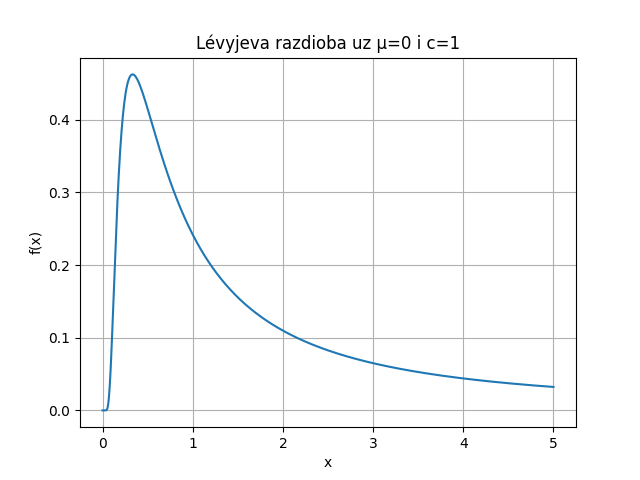
\includegraphics[width=14cm]{levy_dist.png}
	\caption{Graf L\'evyjeve razdiobe za $\mu = 0$ i $c = 1$} 
\end{figure}

Radi jednostavnosti, za određivanje duljine koraka $s$ u L\'evyjevom letu, koristi se sljedeća stabilna razdioba:

\begin{equation}
    L(s) \sim |s|^{-1 - \beta}
\end{equation}
gdje je parametar $\beta \in \langle0, 2]$. Prije upotrebe tu je razdiobu potrebno skalirati.

\begin{figure}[H]
	\centering
	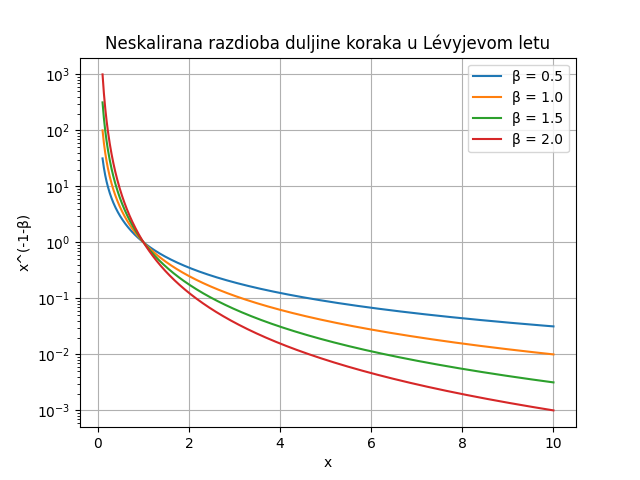
\includegraphics[width=14cm]{levy_step.png}
	\caption{Graf neskalirane razdiobe za L\'evyjev let na logaritamskoj skali} 
\end{figure}


\section{Algoritam}
U samom algoritmu potrebno je idealizirati ponašanje kukavica:
\begin{enumerate}
	\item Kukavice liježu po jedno jaje u nasumično odabrano gnijezdo.
        \item Gnijezda s dobrim jajima (rješenjima) prenose se na sljedeću generaciju.
	\item Broj domaćina je fiksan.
        \item Domaćin može otkriti strano jaje s vjerojatnošću $P_a$.
        \item Ako domaćin otkrije strano jaje, izbacuje ga ili gradi novo gnijezdo na drugoj lokaciji.
\end{enumerate}

Pretpostavlja se $N$ kukavičjih gnijezda u prostoru dimenzije $n$. U svakoj iteraciji algoritma, slučajno odabrana kukavica izvodi 2 radnje:
\begin{enumerate}
    \item Izlegne se i nasumično leti (izvodi L\'evyjev let)
    \item Zamjenjuje slučajno odabrano gnijezdo, ako je na njenom položaju vrijednost funkcije cilja veća
\end{enumerate}

Nakon što se $N$ puta odabere slučajna kukavica, udio od $Pa$ najlošijih gnijezda se izbacuje. Točnije, modificiraju se L\'evyjevim letovima.


\subsection{Kretanje}
Položaj $i$-tu od $N$ kukavica u koraku $t$ predstavlja $n$-dimenzionalni vektor:
\begin{equation}
	\vec{x_i}^t = (x_{i1}^t, x_{i2}^t, \dots, x_{in}^t)
\end{equation}
L\'evyjev let za $i$-tu od $N$ kukavica u koraku $t$ odvija se na sljedeći način:
\begin{equation}
    \vec{x}_i^{t+1} = \vec{x}_i^{t} + \alpha \oplus L(\beta)
\end{equation}
gdje je $\alpha$ faktor skaliranja, a operator $\oplus$ predstavlja međusobno množenje pripadnih elemenata vektora.


\subsection{Pseudokod}


\begin{algorithm}[H]
	\begin{algorithmic}[1]
		\Function{CSA}{obj(x), n, N, Pa, $\alpha$, $\beta$, maxIter}
		
\State x = \Call{InitX}{n, d} \Comment{Inicijalizacija struktura podataka}

  
  \For{iter = 1 to maxIter}

    \For{k = 1 to N}
    \State i = \Call{RandInt}{0, N} \Comment{Slučajan odabir kukavice}
    \State x[i] = x[i] + $\alpha \oplus L(\beta)$  \Comment{L\'evyjev let}
    \State j = \Call{RandInt}{0, N} \Comment{Slučajan odabir gnijezda}
    \If{obj(x[i]) > obj(x[j])}
        \State x[j] = x[i] 
    \EndIf
    \EndFor

    
    \State x = \Call{SortBy}{x, obj}   \Comment{Uzlazno sortiranje po funkciji cilja}
    \For{i = 1 to Pa*N} 
        \State x[i] = x[i] + $\alpha \oplus L(\beta)$ \Comment{Najlošija gnijezda se "izbacuju"}
    \EndFor
    \State x* = \Call{MaxArg}{obj(x)}
  \EndFor
		\State \Return x*	
		\EndFunction
	\end{algorithmic}
	\caption{Algoritam kukavičjeg pretraživanja}
\end{algorithm}









\section{Programsko ostvarenje}

\subsection{Programsko ostvarenje MEALPY}
\hspace{\parindent}Algoritam kukavičjeg pretraživanja ostvaren je u sklopu knjižnice programa otvorenog koda MEALPY\cite{van2023mealpy} programskog jezika Python. Knjižnica je detaljnije opisana u pododjeljku \ref{MP:Bat}.

\hspace{\parindent}Prethodno opisani problem funkcije \eqref{eq:fx} s $n = 10$ definira se u programu kao rječnik i pokreće se algoritam kukavičjeg pretraživanja s 1000 iteracija, brojem šišmiša $N = 50$ i vjerojatnošću otkrivanja $P_a = 0.3$.

\begin{figure}[H]
	\begin{framed}
		\begin{footnotesize}
			\begin{verbatim}
import numpy as np
from mealpy import FloatVar, CSA
from numpy import pi as PI

n = 10

def objective_function(solution):
    return np.sum(solution**2) + 25*np.sum(np.sin(solution)**2)

problem = {
    "obj_func": objective_function,
    "bounds": FloatVar(lb=(-2*PI,)*n, ub=(2*PI,)*n),
    "minmax": "min",
}

model = CSA.OriginalCSA(epoch=1000, pop_size=50, p_a = 0.3)

g_best = model.solve(problem)

print("Solution:", g_best.solution)
print("Fitness:", g_best.target.fitness)			\end{verbatim}
		\end{footnotesize}
	\end{framed}
	\captionof{Kod}{Pokretanje optimizacije vlastite funkcije}
\end{figure}

\begin{figure}[H]
	\begin{framed}
		\begin{footnotesize}
			\begin{verbatim}
Solution: [-0.12270494 -0.92564155 ...  2.82223478]
Fitness: 73.53109251662303
			\end{verbatim}
		\end{footnotesize}
	\end{framed}
	\captionof{Ispis}{Ispis primjera}
\end{figure}



\section{Algoritam kukavičjeg pretraživanja u primjeni}

\subsection{Optimizacija strukture automobilskih dijelova}
\hspace{\parindent} Algoritam kukavičjeg pretraživanja primijenjen je na problem problem optimizacije strukturnog dizajna automobilskih dijelova.\cite{durgun2012} Pokazano je da algoritam pronalazi dobra rješenja. 

\subsection{Pronalazak rubova slika}
\hspace{\parindent} Algoritam je upotrebljen za optimizaciju parametara antecedensa za sustav za pronalaženje rubova utemeljen na Sobelovoj tehnici i neizrazitim intervalima.\cite{7256924} Problem je složen zbog uporabe neizrazitih intervala, stoga se koriste heurističke metode. Zaključeno je da je algoritam kukavičjeg pretraživanja učinkovit za ovakve probleme.

\subsection{Pronalazak štete na mostovima}
\hspace{\parindent} Pronalazak štete na mostovima i gredama problem je koji se rješavao umjetnim neuronskim mrežama.\cite{TRANNGOC2019109637} Učenje težina neuronske mreže algoritmom kukavičjeg pretraživanja bilo je brže i točnije od učenja evolucijskim algoritmom.

\subsection{Modeliranje toka goriva zrakoplova}
\hspace{\parindent} Cilj jednog rada bio je stvaranje modela jačine toka goriva prilikom uspona zrakoplova korištenjem algoritma kukavičjeg pretraživanja.\cite{oruc2020} Jačina toka funkcija je visine i brzine, a korišteni su podaci stvarnog zrakoplova. Takav model bio je u stanju predvidjeti jačinu toka s visokom točnošću. 



\subsection{Diskretni optimizacijski problemi}
\hspace{\parindent} Diskretna inačica algoritma kukavičjeg pretraživanja primijenjena je na niz poznatih diskretnih optimizacijskih problema: TSP, JSSP i QAP.\cite{Ouaarab2020} Dobiveni su rezultati usporedivi s onima srodnih algoritama. 


\subsection{Fuzija slika}
\hspace{\parindent} Fuzija slika je postupak prikupljanja i spajanja bitnih podataka iz više slika. Razvijen je algoritam utemeljen na algoritmu \textit{Grey Wolf} i algoritmu kukavičjeg pretraživanja s rezultatima boljim od ostalih metaheurističkih algoritama.\cite{dutta2020}
